\documentclass[compress, darktitle, framenumber, totalframenumber, handout]{beamer}
\usepackage[greek, dutch]{babel}
\usepackage{booktabs}
\usepackage{manfnt}
\usepackage{marvosym}
\usepackage{mathtools}
\usepackage{pgfplots}
\usepackage{siunitx}
\usepackage{tikz}
\usepackage{wasysym}
\usepackage{wrapfig}
\usepackage{xparse}

\mathtoolsset{showonlyrefs}

\newcommand\frequencydiagram[5]{
  % TODO change number of samples
  \begin{tikzpicture}[scale = 0.85, domain = 0:10, samples = 1000]
    \draw[very thin] (-0.1,-2.1) grid (10.1,2.1);
    \draw[thick, ->] (-0.2,0) -- (10.2,0);

    \draw[fill] (0,0) circle (2pt) node [below left] {$0$};
    \draw[fill] (pi,0) circle (2pt) node [below] {$\pi$};
    \draw[fill] (2*pi,0) circle (2pt) node [below] {$2\pi$};
    \draw[fill] (3*pi,0) circle (2pt) node [below] {$3\pi$};

    \draw[color = vividbrown] plot function{sin(#1*#2*x)} node[right] {\SI{#4}{\hertz}};
    \draw[color = uared] plot function{sin(#1*#3*x)} node[right] {\SI{#5}{\hertz}};

    \pause
    \draw[color = vividbrown!40] plot function{sin(#1*#2*x)} node[right] {\SI{#4}{\hertz}};
    \draw[color = uared!40] plot function{sin(#1*#3*x)} node[right] {\SI{#5}{\hertz}};
    \draw[semithick, color = uablue] plot function{2*sin(#1*(#3+#2)*x/2)*cos(#1*(#3-#2)*x/2)} node[right] {som};
  \end{tikzpicture}
}

\usetheme{UniversiteitAntwerpen}
\beamertemplatenavigationsymbolsempty

\newtranslation[to=dutch]{Section}{Deel}
\AtBeginSection{\frame{\sectionpage}}

\newenvironment{danger}{\medbreak\noindent\hangindent=2pc\hangafter=-2%
  \clubpenalty=10000%
  \hbox to0pt{\hskip-\hangindent\dbend\hfill}\small\ignorespaces}%
  {\medbreak\par}

\title{Wisku$\mathbb{N}$de in-$\mathbb{Z}$icht}
\subtitle{Wiskunde in muziek}
\author{Pieter Belmans (\texttt{pieter.belmans@uantwerpen.be}) \\ Matthias Roels (\texttt{matthias.roels@uantwerpen.be})}
\date{9 of 14 januari 2014}

\begin{document}
\begin{frame}
  \titlepage
\end{frame}

\begin{frame}
  \frametitle{Wat gaan we vandaag doen?}

  \begin{block}{Voormiddag}
    \begin{wrapfigure}{r}{.5\textwidth}
      \centering
      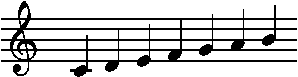
\includegraphics{scores/scale-cropped}
    \end{wrapfigure}
    Waarom do-re-mi-fa-sol-la-si?
    \begin{enumerate}
      \item de structuur van geluid
      \item mooi en lelijk
      \item 7 (of 12) noten
    \end{enumerate}
  \end{block}

  \pause

  \begin{block}{Namiddag}
    Wat maakt geluid muziek?
    \begin{enumerate}
      \item de structuur van geluid analyseren
      \item voorbeelden
      \item verschillen tussen muziekinstrumenten
    \end{enumerate}
  \end{block}
\end{frame}

\begin{frame}
  \frametitle{Vragen staat vrij}

  Voorkennis (?):
  \begin{enumerate}
    \item de sinus
    \item goniometrische formules
    \item rekenen met logaritmes
    \item muziek: noten lezen, enige terminologie
  \end{enumerate}
\end{frame}


\section{Wat zijn boventonen?}
% TODO refer to last part of talk, and afternoon

\begin{frame}
  \frametitle{Wat is geluid?}

  Geluid is een \emph{golf}: een verandering in de luchtdruk.
  \pause
  \begin{enumerate}
    \item Hoe kunnen we geluid analyseren?
    \item Hoe kunnen we onze analyse interpreteren?
  \end{enumerate}
  \pause
  We willen dus
  \begin{enumerate}
    \item de bouwstenen van geluid kennen;
    \item weten hoe we deze bouwstenen kunnen combineren;
    \item van een specifiek geluid de bouwstenen bepalen.
  \end{enumerate}
\end{frame}

\begin{frame}
  \frametitle{Staande golven}

  \begin{block}{\Forward\ filmfragment}
    \url{http://www.youtube.com/watch?v=-n1d1rycvj4}
  \end{block}

  \pause

  Als we een periodiek signaal geven, met een geheel veelvoud van de frequentie waarmee het langsheen het touw reist, krijgen we een \alert{staande golf}: deze versterkt zichzelf.
\end{frame}

\begin{frame}
  \frametitle{Boventonen}

  \centering
  \begin{tikzpicture}[scale = .7]
    \foreach \k in {1,...,7} {
      \draw[smooth, domain = 0:3*pi, samples = 100] plot (\x,{sin(60*\k*\x/pi)/5-\k});
      \draw[smooth, domain = 0:3*pi, samples = 100] plot (\x,{-sin(60*\k*\x/pi)/5-\k});
      \draw[fill] (0,-\k) circle (1pt);
      \draw[fill] (3*pi,-\k) circle (1pt);
    };

    \draw (3*pi,-1) node[above, uablue, font = \tiny] {$1$};
    \foreach \k in {2,...,7} {
      \draw[fill, uablue!60] (3*pi/\k,-\k) circle (1pt) node[above, uablue, font = \tiny] {$1/\k$};
    };
  \end{tikzpicture}
\end{frame}

\begin{frame}
  \frametitle{Fundamentele grondtoon}

  De frequentie van de grondtoon van een snaar wordt gegeven door de \alert{wet van Mersenne}
  \begin{equation}
    f_0=\frac{1}{2L}\sqrt{\frac{T}{\mu}}
  \end{equation}
  waarbij
  \begin{equation}
    \begin{aligned}
      L&=\text{lengte van de snaar} \\
      T&=\text{spanning op de snaar (= kracht)} \\
      \mu&=\text{massa per lengte}
    \end{aligned}
  \end{equation}
  \pause
  \begin{block}{Voorbeeld}
    $L=\SI{65}{\centi\meter}$, $T=\SI{83}{\newton}\approx\SI{8.5}{\kilo\gram}$, $\mu\approx\SI{0.74}{\gram\per\meter}$ \\
    $\Rightarrow f_0\approx\SI{83}{\hertz}$ en dit is de lage mi op een gitaar
  \end{block}
\end{frame}

\begin{frame}
  \frametitle{Het menselijk gehoor}

  Wij zijn ruwweg in staat om geluid tussen $\SI{20}{\hertz}$ en $\SI{20}{\kilo\hertz}$ te horen.
  \pause
  \begin{enumerate}
    \item menselijke stem: $85$ tot $\SI{180}{\hertz}$ voor mannen, $165$ tot $\SI{255}{\hertz}$ voor vrouwen;
    \pause\item viool $\SI{196}{\hertz}$ tot $\pm\SI{4.5}{\kilo\hertz}$;
    \pause\item gitaar: $\SI{83}{\hertz}$ tot $\SI{\pm 1}{\kilo\hertz}$;
    \pause\item piano: $\SI{27}{\hertz}$ tot $\SI{4.2}{\kilo\hertz}$.
  \end{enumerate}
  \pause
  Dit is de frequentie van de \alert{grondtoon}. Stem of muziek is \emph{veel meer dan dit}! Maar voor onze perceptie van ``toonhoogte'' is deze frequentie wel essentieel.
\end{frame}

\begin{frame}
  \frametitle{Boventonen in snaren}

  Als we aan een snaar trekken gaat die in het wilde weg trillen, om vervolgens te gaan trillen met:
  \begin{enumerate}
    \item met de frequentie van de grondtoon,
    \item met de frequentie van de boventonen
  \end{enumerate}
  want deze versterken zich door het fenomeen van de staande golf, terwijl de andere frequenties grotendeels verdwijnen.
  \pause
  \begin{block}{Experiment}
    \begin{enumerate}
      \item een losse snaar;
        \pause
      \item we halveren de snaar: harmoniek vs.\ fret
        \pause
      \item we delen de snaar in drie: harmoniek vs.\ fret
    \end{enumerate}
  \end{block}
\end{frame}

\begin{frame}
  \frametitle{Boventonen}

  \centering
  \begin{tikzpicture}[scale = .7]
    \foreach \k in {1,...,7} {
      \draw[smooth, domain = 0:3*pi, samples = 100] plot (\x,{sin(60*\k*\x/pi)/5-\k});
      \draw[smooth, domain = 0:3*pi, samples = 100] plot (\x,{-sin(60*\k*\x/pi)/5-\k});
      \draw[fill] (0,-\k) circle (1pt);
      \draw[fill] (3*pi,-\k) circle (1pt);
    };

    \draw (3*pi,-1) node[above, uablue, font = \tiny] {$1$};
    \foreach \k in {2,...,7} {
      \draw[fill, uablue!60] (3*pi/\k,-\k) circle (1pt) node[above, uablue, font = \tiny] {$1/\k$};
    };
  \end{tikzpicture}
\end{frame}


\section{Wat klinkt er mooi samen en wat niet?}

\begin{frame}
  \frametitle{We luisteren naar boventonen}

  De boventonen hebben een sterk verband met de grondtoon, en geven een mooie samenklank.

  \pause

  Als sinussen:
  \begin{block}{\twonotes\ audiofragmenten}
    \texttt{samples/440-880.mp3} \\
    \texttt{samples/440-880-878.mp3} \\
  \end{block}

  \pause
  Conclusie:
  \begin{enumerate}
    \item gehele veelvouden klinken mooi samen
    \item n\'et niet gehele veelvouden klinken lelijk
  \end{enumerate}
\end{frame}

\begin{frame}
  \frametitle{Nu met echte instrumenten}

  \begin{block}{Experiment}
    \begin{enumerate}
      \item octaaf ($2:1$)
        \pause
      \item kwint ($3:2$)
        \pause
      \item septiem ($15:8$)
        \pause
      \item kleine sixt ($11:7$)
    \end{enumerate}
  \end{block}

  \pause

  \begin{alertblock}{Conclusie}
    Ons gehoor houdt van gehele veelvouden en verhoudingen van kleine getallen.
  \end{alertblock}
\end{frame}

\begin{frame}
  \frametitle{Het samen laten klinken van twee geluidsgolven}

  Wat gebeurt er als we twee frequenties~$f_1$ en~$f_2$ laten horen?
  \begin{equation}
    \sin(f_1t)+\sin(f_2t)=\onslide<1>{?}\pause\!\!\!2\sin\left( \frac{f_1+f_2}{2}t \right)\cos\left( \frac{f_1-f_2}{2}t \right).
  \end{equation}

  \pause

  Welke conclusies zijn er te trekken?

  \pause

  \begin{enumerate}
    \item de factor 2 levert ons dat het signaal tot dubbel zo sterk kan worden;
    \item de sinus of cosinus in het product kan 0 zijn.
  \end{enumerate}

\end{frame}

\begin{frame}
  \frametitle{Voorbeeld}

  Stel $f_1=\SI{2}{\hertz}$ en $f_2=\SI{3}{\hertz}$:

  \begin{center}
    \frequencydiagram{2}{1}{1.5}{2}{3}
  \end{center}

  \onslide<2>{Soms versterken de twee signalen elkaar, soms verzwakken ze elkaar.}
\end{frame}

\begin{frame}
  \frametitle{Voorbeeld}

  Stel $f_1=\SI{3}{\hertz}$ en $f_2=\SI{4}{\hertz}$:

  \begin{center}
    \frequencydiagram{3}{1}{1.3333}{3}{4}
  \end{center}

  \onslide<2>{Het versterken en verzwakken is (uiteraard) ook periodisch.}
\end{frame}

\begin{frame}
  \frametitle{Voorbeeld}

  Stel $f_1=\SI{3}{\hertz}$ en $f_2=\SI{5}{\hertz}$:

  \begin{center}
    \frequencydiagram{3}{1}{1.666}{3}{5}
  \end{center}

  \onslide<2>{Golven kunnen \alert{in fase} of \alert{uit fase} zijn.}
\end{frame}

\begin{frame}
  \frametitle{Zweving}

  Wat als~$f_1$ en~$f_2$ bijna hetzelfde zijn?
  
  Stel $f_1=\SI{8}{\hertz}$, $f_2=\SI{9}{\hertz}$:

  \begin{center}
    \frequencydiagram{8}{1}{1.125}{8}{9}
  \end{center}
\end{frame}

\begin{frame}
  \frametitle{Nog meer zweving}

  Stel $f_1=\SI{16}{\hertz}$, $f_2=\SI{17}{\hertz}$:

  \begin{center}
    \frequencydiagram{16}{1}{1.0625}{16}{17}
  \end{center}

  \onslide<2>{We zien opnieuw een golfpatroon met frequentie $\SI{1}{\hertz}=\SI{17}{\hertz}-\SI{16}{\hertz}$}
\end{frame}

\begin{frame}
  \frametitle{Zweving}

  \begin{block}{\twonotes\ audiofragmenten}
    \texttt{samples/440-880-878.mp3} \\
    experiment
  \end{block}

  \pause

  \begin{alertblock}{Definitie}
    Het luider en stiller worden van het geluid noemen we \emph{zweving} (of \emph{beating} in het Engels).
  \end{alertblock}

  \begin{enumerate}
    \item instrumenten die niet goed gestemd zijn geven zulke zwevingen
    \item zweving kan best vermeden worden (maar soms is het intentioneel, zeker in moderne muziek)
  \end{enumerate}
\end{frame}


\section{Hoe maken we verschillende noten?}

\begin{frame}
  \frametitle{Gehele veelvouden}

  Muziek met 1 noot zou maar saai zijn. Hoe kiezen we de andere noten? \pause We willen
  \begin{enumerate}
    \item mooie samenklank
    \item \pause genoeg noten om interessante muziek te schrijven
    \item \pause niet te veel noten om de muziek nog speelbaar te houden
  \end{enumerate}

  We hebben een goede leidraad voor mogelijke nieuwe noten: de \alert{boventonen}! De eerste voorwaarde is alvast voldaan.

  Hoe gaan we verder?
\end{frame}

\begin{frame}
  \frametitle{De kwint}

  De \alert{tweede boventoon} ``klinkt hetzelfde'', de verdubbeling in frequentie levert geen echt verschil op, we noemen dit een \alert{octaaf}.
  \pause
  Om hem te spelen op een snaar moeten we de snaarlengte \emph{halveren}.
  \begin{block}{Experiment}
    halveer de snaarlengte
  \end{block}

  \pause

  De \alert{derde boventoon} (dus 3 maal de grondfrequentie) is w\'el anders!

  \begin{enumerate}
    \item De snaar \emph{in drie delen} levert deze frequentie als grondtoon.
    \item \pause De lengte verdubbelen geeft $3/2$ keer de grondfrequentie.
  \end{enumerate}
  \begin{block}{Experiment}
    1/3 en 2/3 van de snaarlengte
  \end{block}
  \pause
  Het resultaat noemen we een \alert{kwint}.
\end{frame}

\begin{frame}
  \frametitle{Octaven en kwinten}

  We horen nu de grondtonen met frequenties $\SI{220}{\hertz}$ (= la) en $\SI{330}{\hertz}$ (= mi)
  \begin{block}{\twonotes\ audiofragmenten}
    \begin{wrapfigure}{r}{.4\textwidth}
      \vspace{-.5cm} % weird hack to get position right
      \centering
      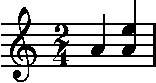
\includegraphics{scores/fifths-cropped}
    \end{wrapfigure}

    % TODO these should be made with a real piano sound!
    \texttt{samples/octave.mp3} \\
    \texttt{samples/fifth.mp3} \\
    \texttt{samples/octave-fifth.mp3}
  \end{block}
\end{frame}

\begin{frame}
  \frametitle{Kwinten visueel}

  \begin{center}
    \frequencydiagram{22}{1}{1.5}{22}{33}
  \end{center}
\end{frame}

\begin{frame}
  \frametitle{Kwinten visueel}

  Wat als we net geen verhouding van $3/2$ hebben?
  \begin{center}
    \frequencydiagram{22}{1}{1.5454}{22}{34}
  \end{center}
  \pause
  We zien \alert{zweving} optreden.
\end{frame}

\begin{frame}
  \frametitle{De terts}

  De \alert{vierde boventoon} is een verviervoudiging van de grondfrequentie, dus \alert{twee octaven}.

  \pause
  \vspace{1em}

  De \alert{vijfde boventoon} is w\'el nieuw. We hebben $5/4$ keer de grondfrequentie.

  \begin{block}{Experiment}
    \begin{wrapfigure}{r}{.4\textwidth}
      \vspace{-.5cm} % weird hack to get position right
      \centering
      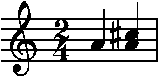
\includegraphics{scores/thirds-cropped}
    \end{wrapfigure}
    (grote) tertsen door 4/5 van de snaarlengte te spelen \\
    \pause we hebben ook de harmonieken van de terts door 1/5 van de snaarlengte af te dempen
  \end{block}
  \pause
  Merk op, de fretten van een gitaar staan steeds dichter bij elkaar.
\end{frame}

\begin{frame}
  \frametitle{Octaven, kwinten en tertsen}

  We horen nu de grondtonen met frequenties $\SI{220}{\hertz}$ (= la), $\SI{275}{\hertz}$ (= do\#) en $\SI{330}{\hertz}$ (= mi)
  \begin{block}{\twonotes\ audiofragmenten}
    \begin{wrapfigure}{r}{.4\textwidth}
      \vspace{-.5cm} % weird hack to get position right
      \centering
      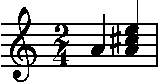
\includegraphics{scores/major-chord-cropped}
    \end{wrapfigure}

    \texttt{samples/thirds.mp3} \\
    \texttt{samples/fifths-thirds.mp3} \\
    \texttt{samples/major-chord.mp3}
  \end{block}

  \pause

  We misbruiken hier natuurlijk de notatie die we pas kunnen invoeren als we het systeem volledig bedacht hebben.
\end{frame}

\begin{frame}
  \frametitle{Een toonladder bouwen}

  We hebben nu de basis voor onze muziek in handen:
  \begin{enumerate}
    \item kwinten;
    \item tertsen.
  \end{enumerate}
  We kunnen deze stapelen, om zo nieuwe noten te vormen.
  \pause
  \begin{itemize}
    \item \hyperlinkslidenext{\beamergotobutton{doe het historisch intermezzo}}
    \item \hyperlink{tunings}{\beamerskipbutton{sla het historisch intermezzo over}}
  \end{itemize}
\end{frame}


\section{Een historisch intermezzo}

\begin{frame}[label=history]
  \frametitle{Musica universalis}

  Pythagoras:
  \begin{enumerate}
    \item toonhoogte staat in verband met de lengte van een snaar
    \item de 7 hemellichamen volgen dezelfde regels
  \end{enumerate}

  \pause
  Voor hem waren muziektheorie en astronomie nauw verbonden:
  \begin{enumerate}
    \item astronomie is \alert{zichtbare} regelmaat,
    \item muziek is \alert{hoorbare} regelmaat,
  \end{enumerate}
  en beiden gaan over \alert{``perfecte'' verhoudingen}.
\end{frame}

\begin{frame}
  \frametitle{Musica universalis}

  \begin{block}{Plinius de oudere, Naturalis Historia, 77--79 n.C.}
    Sed Pythagoras interdum et musica ratione appellat quantum absit a terra luna, ab ea ad Mercurium dimidium spatii et ab eo ad Veneris, a quo ad solem sescuplum, a sole ad Martem tonum [id est quantum ad lunam a terra], ab eo ad Iovem dimidium et ab eo ad Saturni, et inde sescuplum ad signiferum; ita septem tonis effici quam \greektext di`a paswn 'armon'ian \latintext hoc est universitatem concentus; in ea Saturnum Dorio moveri phthongo, Iovem Phrygio et in reliquis similia, iucunda magis quam necessaria subtilitate.
  \end{block}

  \pause

  Dit \alert{geocentrisch model} is natuurlijk onzin.
\end{frame}

\begin{frame}[plain]
  \centering
  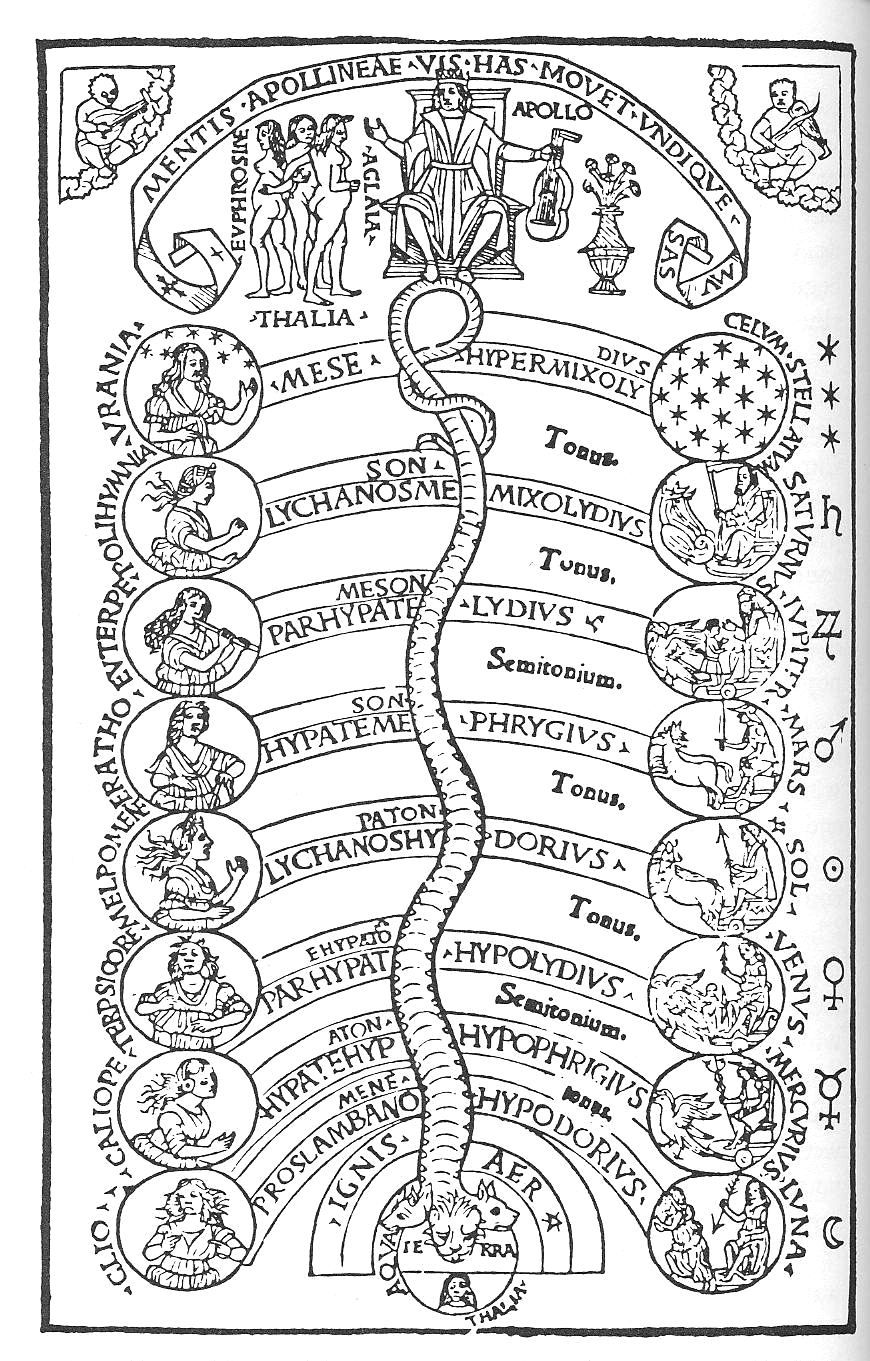
\includegraphics[width=6cm]{images/spheres}
\end{frame}

\begin{frame}
  \frametitle{Baanresonantie}

  \begin{block}{Pythagoras had overigens gelijk}
    Sommige hemellichamen bewegen w\'el in een mooie verhouding:
    \begin{enumerate}
      \item Pluto--Neptunus: $3:2$
      \item Io--Europa--Ganymedes (manen van Jupiter): $4:2:1$
    \end{enumerate}
  \end{block}

  \pause

  \begin{alertblock}{Chronologie}
    \begin{danger}
      Maar geen van deze objecten was reeds ontdekt ten tijde van Pythagoras! Laat staan zichtbaar zonder telescopen.
    \end{danger}
  \end{alertblock}
\end{frame}

\section{Wat is het probleem met stemmingen?}

\begin{frame}[label=tunings]
  \frametitle{Een stemming}

  We moeten dus toonhoogtes afspreken die we zullen gebruiken om muziek te maken. We weten dat
  \begin{enumerate}
    \item gehele veelvouden en kleine breuken goed klinken;
    \item we zweving moeten vermijden;
    \item de kwint (en de terts) interessante bouwblokken zijn.
  \end{enumerate}
  \pause
  We willen dus:
  \begin{enumerate}
    \item mooie kwinten en tertsen
    \item genoeg noten om interessante muziek te kunnen maken
    \item niet te veel noten om het niet te moeilijk te maken
  \end{enumerate}
\end{frame}

\begin{frame}
  \frametitle{De kwint als bouwblok}

  We zullen kwinten stapelen:
  \begin{enumerate}
    \item elke stap apart klinkt mooi samen
    \item het houdt verband met de tertsen: 5e versus 3e (= 6e) boventoon: na 4 kwinten (= 30e boventoon) hebben we een veelvoud van de 5e boventoon bereikt
  \end{enumerate}
\end{frame}

\begin{frame}
  \frametitle{Dezelfde noot, of toch niet?}

  Neem een grondnoot (bijvoorbeeld de do), en beschouw
  \begin{enumerate}
    \item 7 octaven erboven: opnieuw een do
      \pause
    \item 12 kwinten erboven: \alert{kwintencirkel} \\
      do sol re la mi si fa\# do\# sol\# re\# la\# mi\# si\#

      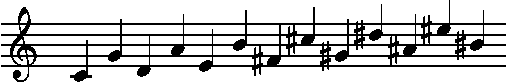
\includegraphics{scores/circle-cropped}
  \end{enumerate}
  \pause
  in frequenties:
  \begin{description}
    \item[grondnoot:] $\SI{100}{\hertz}$ (om de getallen mooier te maken!)
    \item[7 octaven:] $2^7\cdot\SI{100}{\hertz}=\SI{12800}{\hertz}$ 
      \pause
    \item[12 kwinten:] $(3/2)^{12}\cdot\SI{100}{\hertz}\approx\SI{12975}{\hertz}$
  \end{description}
\end{frame}

\begin{frame}
  \frametitle{Dezelfde noot: si\# = do}

  We brengen alles 7 octaven naar beneden:
  \begin{description}
    \item[grondnoot:] $\SI{100}{\hertz}$
    \item[12 kwinten:] $(3/2)^{12}/2^7\cdot\SI{100}{\hertz}\approx\SI{101.36}{\hertz}$
  \end{description}
  \pause
  \begin{block}{\twonotes\ audiofragment}
    \texttt{samples/7-12-glissando-400Hz.mp3} \\
    \texttt{samples/7-12-400Hz.mp3}
  \end{block}
  \pause
  We willen (?) si\# = do zodat we slechts 12 noten moeten gebruiken in onze muziek.

  \begin{alertblock}{Vraag}
    Is dit de enige mogelijke keuze?
  \end{alertblock}
\end{frame}

\begin{frame}
  \frametitle{Waarom het nooit kan kloppen}

  \begin{block}{Antwoord}
    Dit is niet de enige mogelijke keuze!
  \end{block}
  We bouwen onze toonladder op met behulp van octaven en kwinten. En we willen op een bepaald moment twee noten gelijkstellen.

  \pause
  Dat betekent:
  \begin{equation}
    2^n=\left( \frac{3}{2} \right)^m
  \end{equation}
  voor~$m$ en~$n$ natuurlijke getallen. Op de vorige slide: $n=7,m=12$.
  \pause
  \begin{alertblock}{Vraag}
    Zijn er perfecte keuzes mogelijk?
  \end{alertblock}
\end{frame}

\begin{frame}
  \frametitle{Waarom het nooit kan kloppen}

  \begin{block}{Antwoord}
    Nee!
  \end{block}
  \pause
  \begin{equation}
    \begin{aligned}
      2^n=\left( \frac{3}{2} \right)^m&\Longleftrightarrow 2^{n+m}=3^m
    \end{aligned}
  \end{equation}
  maar het linkerlid is even, het rechterlid oneven.
  \pause
  \begin{block}{Onoplosbaar}
    Dit probleem is niet op te lossen, en hangt nu eenmaal af van onze keuze om si kruis en do gelijk te stellen.
  \end{block}
  We zullen daarom gewoon beginnen bouwen, en zien waar het misloopt.
\end{frame}

\begin{frame}
  \frametitle{We bouwen onze toonladder}

  We bouwen een toonladder met als basis de kwint $3:2$ en terts $5:4$
  \begin{center}
    \begin{tabular}{ccccccccc}
      noot & do & re & mi & fa & sol & la & si & do \\
      verhouding & $1:1$ & \onslide<3->{$9:8$} & $5:4$ & \onslide<2->{$4:3$} & $3:2$ & \onslide<4->{$5:3$} & \onslide<5->{$15:8$} & $2:1$
    \end{tabular}
  \end{center}
  \begin{enumerate}
    \item<2-> fa is omgekeerde kwint, $(3:2)^{-1}=(4:3)$
    \item<3-> re is twee kwinten, $(3:2)^2=(9:8)$ (we negeren octaven)
    \item<4-> la is kleine terts naar beneden (= kwint min grote terts), $((3:2)(5:4)^{-1})^{-1}=(5:3)$
    \item<5-> si is grote terts boven kwint, $(3:2)(5:4)=(15:8)$
  \end{enumerate}

  \onslide<6->{Door wiskunde te gebruiken kunnen we heel makkelijk rekenen met intervallen!}
\end{frame}

\begin{frame}
  \frametitle{Wat is er mis met deze toonladder?}

  We hebben si\# = do genomen: \alert{enharmonie}.
  \pause
  Maar daardoor gaan bepaalde (enharmonische) intervallen niet meer juist klinken\ldots
  \pause
  \begin{block}{Voorbeeld van een wolfinterval}
    De elf kwinten zijn perfect gekozen (want exact $3:2$), de twaalfde kwint is dus significant te klein.
  \end{block}
  \pause
  Er is nog een ander probleem.
  \begin{block}{Voorbeeld van problemen met stapelen}
    \begin{itemize}
      \item de sixt in do groot: $5:3$
      \item de seconde in sol groot: $9:8$, en dus $(3:2)(9:8)=27:16$ tegenover do
    \end{itemize}
    We kunnen dus niet zomaar moduleren!
  \end{block}
\end{frame}

\section{Rekenen met toonhoogtes}

\begin{frame}
  \frametitle{Frequenties zijn onhandig}

  Het rekenen met frequenties is een \alert{absolute} manier van werken. \pause De problemen:
  \begin{enumerate}
    \item afhankelijk van de gekozen basisfrequentie (tegenwoordig $\SI{440}{\hertz}$);
    \item afhankelijk van de gekozen octaaf;
    \item onhandig rekenen: we werken met een \alert{exponenti\"ele schaal}, terwijl het aantal noten wel constant blijft
  \end{enumerate}
  \begin{center}
    \begin{tikzpicture}
      \foreach \k in {0,...,36} \draw [fill] ({exp(1+\k/12)/3},0) circle (.5pt);
      \foreach \k in {0,1,2,3} \draw [fill] ({exp(1+\k)/3},0) circle (1pt) node [below] {do};
      \foreach \k in {0,1,2} \draw [fill, uared] ({exp(1+\k+5/12)/3},0) circle (1pt) node [below] {fa};
      \foreach \k in {0,1,2} \draw [fill, uared] ({exp(1+\k+7/12)/3},0) circle (1pt) node [below] {sol};
    \end{tikzpicture}
  \end{center}
\end{frame}

\begin{frame}
  \frametitle{Het alternatief}
  
  Daarom willen we een \alert{relatieve} manier van werken!
  \begin{enumerate}
    \item onafhankelijk van octaaf en basisfrequentie;
    \item een \alert{lineaire schaal}
  \end{enumerate}
  \begin{center}
    \begin{tikzpicture}
      \foreach \k in {0,...,36} \draw [fill] ({\k/6},0) circle (.5pt);
      \foreach \k in {0,1,2,3} \draw [fill] ({12*\k/6},0) circle (1pt) node [below] {do};
      \foreach \k in {0,1,2} \draw [fill, uared] ({(12*\k+7)/6},0) circle (1pt) node [below] {sol};
    \end{tikzpicture}
  \end{center}
\end{frame}

\begin{frame}
  \frametitle{Cents}

  We zullen een octaaf in 12 gelijke delen (exponentieel gezien) opdelen (we weten nog niet waarom!). Daarom: stel $f_1$ en~$f_2$ de frequenties van twee noten, dan is
  \begin{equation}
    1200\cdot\log_2\left( \frac{f_2}{f_1} \right)=1200\cdot\left( \log_2(f_2)-\log_2(f_1) \right)
  \end{equation}
  het aantal \alert{cent} van $f_1$ naar $f_2$.
  \pause
  De toonladder wordt dus
  \begin{center}
    \begin{tikzpicture}
      \draw (0,0) circle (.1pt) node [above] {\small 0 cent};
      \draw (5/2,0) circle (.1pt) node [above, xshift = -5pt] {\small 500 cent};
      \draw (7/2,0) circle (.1pt) node [above, xshift = 15pt] {\small 700 cent};
      \draw (12/2,0) circle (.1pt) node [above] {\small 1200 cent};
      \foreach \k in {0,...,12} \draw [fill] ({\k/2},0) circle (.5pt);
      \foreach \k in {0,1} \draw [fill] ({12*\k/2},0) circle (1pt) node [below] {do};
      \foreach \k in {0} \draw [fill, uared] ({(12*\k+7)/2},0) circle (1pt) node [below] {sol};
      \foreach \k in {0} \draw [fill, uared] ({(12*\k+5)/2},0) circle (1pt) node [below] {fa};
    \end{tikzpicture}
  \end{center}
  \pause
  in plaats van
  \begin{center}
    \begin{tikzpicture}
      \draw ({exp(1+0/12)*1.5},0) circle (.1pt) node [above] {\small $\SI{130.81}{\hertz}$};
      \draw ({exp(1+5/12)*1.5},0) circle (.1pt) node [above, xshift = -5pt] {\small $\SI{174.61}{\hertz}$};
      \draw ({exp(1+7/12)*1.5},0) circle (.1pt) node [above, xshift = 10pt] {\small $\SI{196}{\hertz}$};
      \draw ({exp(1+12/12)*1.5},0) circle (.1pt) node [above] {\small $\SI{261.63}{\hertz}$};
      \foreach \k in {0,...,12} \draw [fill] ({exp(1+\k/12)*1.5},0) circle (.5pt);
      \foreach \k in {0,1} \draw [fill] ({exp(1+\k)*1.5},0) circle (1pt) node [below] {do};
      \foreach \k in {0} \draw [fill, uared] ({exp(1+\k+5/12)*1.5},0) circle (1pt) node [below] {fa};
      \foreach \k in {0} \draw [fill, uared] ({exp(1+\k+7/12)*1.5},0) circle (1pt) node [below] {sol};
    \end{tikzpicture}
  \end{center}
\end{frame}


\section{Hoe kunnen we ons probleem oplossen?}
\begin{frame}
  \frametitle{Geschiedenis}

  De scenario's:
  \begin{description}[middeleeuwen]
    \item[Pythagoras] strak vasthouden aan de perfecte verhoudingen, goed in theorie, slecht in praktijk
    \item[middeleeuwen] variaties op Pythagoras: het ``wolfinterval'' dat ontstaat door de strikte toepassing van Pythagoras' theorie wordt uitgesmeerd over meerdere noten
    \item[hedendaags] we nemen gelijke stappen, de \alert{gelijkzwevende stemming}
  \end{description}
  \pause
  \begin{block}{Chronologie gelijkzwevende stemming}
    \begin{enumerate}
      \item 4e eeuw voor Christus: Aristoxenus
      \item 1584: Vincenzo Galilei (vader van)
      \item 1605: Simon Stevin (Belgisch wiskundige!) beschrijft voor het eerst de huidige stemming, \emph{Van de Spiegeling der singconst}
      \item \ldots
    \end{enumerate}
  \end{block}
\end{frame}

\begin{frame}
  \frametitle{Hoeveel noten hebben we nodig?}

  \begin{center}
    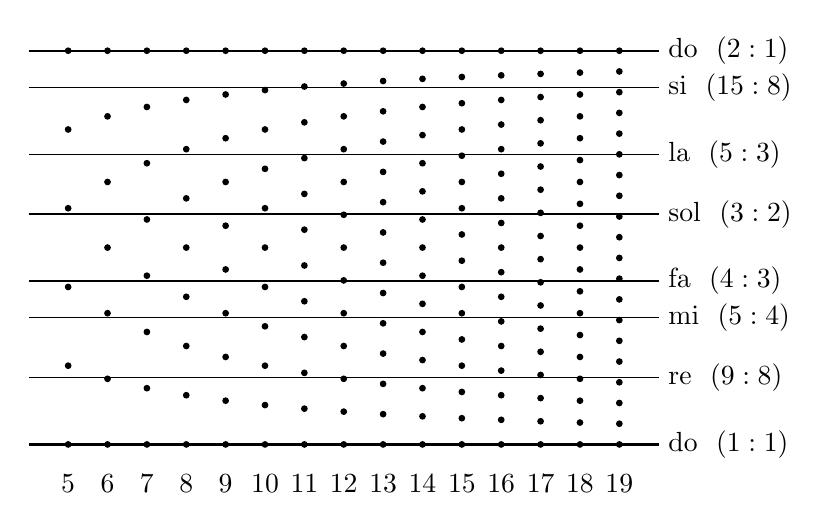
\begin{tikzpicture}
      \foreach \t/\n/\name in {1/1/do, 9/8/re, 5/4/mi, 4/3/fa, 3/2/sol, 5/3/la, 15/8/si, 2/1/do} {
        \draw (2, {5*ln(\t/\n)/ln(2)}) --++ (8, 0) node[right] {\name\ \ $(\t:\n)$};
      };
      \draw[thick] (2, {5*ln(3/2)/ln(2)}) --++ (8, 0);
      \draw[thick] (2, {5*ln(1/1)/ln(2)}) --++ (8, 0);
      \draw[thick] (2, {5*ln(2/1)/ln(2)}) --++ (8, 0);
  
      \foreach \k in {5,...,19} {
        \draw (\k/2,-.5) node {\k};
        \foreach \m in {0,...,\k} {
          \draw[fill] (\k/2, 5*\m/\k) circle (1pt);
        };
      };
    \end{tikzpicture}
  \end{center}
\end{frame}

\begin{frame}
  \frametitle{Grootte van de fout}

  \begin{center}
    \begin{tikzpicture}
      \begin{axis}[width = \textwidth, height = .9\textheight, ytick=\empty, xlabel = {aantal noten}, ylabel = {cumulatieve fout}, xtick pos = left]
        \addplot[uablue, mark = *] table {error.dat};
      \end{axis}
    \end{tikzpicture}
  \end{center}
\end{frame}

\begin{frame}
  \frametitle{Daarom do-re-mi-fa-sol-la-si!}

  \begin{block}{Conclusie}
    We zien dat \alert{12 gelijke tonen} de volgende eigenschappen heeft:
    \begin{enumerate}
      \item bijna perfecte kwint, kwart, seconde
      \item alles is regelmatig
      \item niet te veel noten
      \item het staat (toevallig?) in verband met de 12 kwinten: de \emph{minimale} keuze voldoet blijkbaar (als we niet al te veeleisend zijn)
    \end{enumerate}
  \end{block}
\end{frame}

\begin{frame}
  \frametitle{Gelijkzwevende vs.\ reine stemming}

  Hoe verhoudt deze gelijkzwevende stemming zich nu tot de ``natuurlijke'' of reine stemming?
  \pause
  \begin{description}
    \item[kwint] $3:2$ vs.\ $2^{7/12}$ \\
      \pause= $1.5$ vs.\ $1.4983\dotso$ \\
      \pause= $701.955\dotso$ cent vs.\ $700$ cent
    \item[terts] $5:4$ vs.\ $2^{4/12}$ \\
      \pause= $1.25$ vs.\ $1.2599\dotso$ \\
      \pause= $386.313$\dotso cent vs.\ $400$ cent
  \end{description}
  \begin{block}{Vuistregel}
    Goede muzikanten horen een verschil vanaf 5 cent.
  \end{block}
  Wanneer twee noten tegelijkertijd gespeeld worden en er zweving kan worden vastgesteld is het natuurlijk gemakkelijker.
\end{frame}


\section{Hoe kan geluid ons bedotten?}
\begin{frame}
  \frametitle{Illusies met geluid}

  % http://tex.stackexchange.com/questions/129274/showcase-of-optical-illusions-made-with-tex-latex-luatex-context
  \centering
  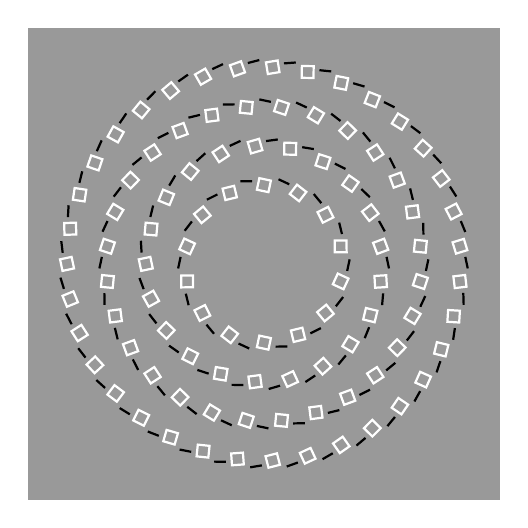
\begin{tikzpicture}[scale = .5]
    \fill[color=black!40!white] (-6,-6) rectangle (6,6);
    \foreach \n/\r/\twist in {70/5/12,56/4/-12,42/3/12,28/2/-12}{
      \foreach \m in {1,3,...,\n}
        \draw [thick,color=white,shift={(360/\n*\m:\r)},rotate=\twist+360/\n*\m] (-.15,-.15) rectangle (.15,.15);
      \foreach \m in {2,4,...,\n}
        \draw [thick,color=black,shift={(360/\n*\m:\r)},rotate=\twist+360/\n*\m] (.15,-.15) rectangle (.15,.15);
      }
  \end{tikzpicture}
\end{frame}

\begin{frame}
  \frametitle{Een toonladder}

  \begin{block}{\twonotes\ audiofragment}
    \texttt{samples/endless.mp3}
  \end{block}
  \pause
  \begin{center}
    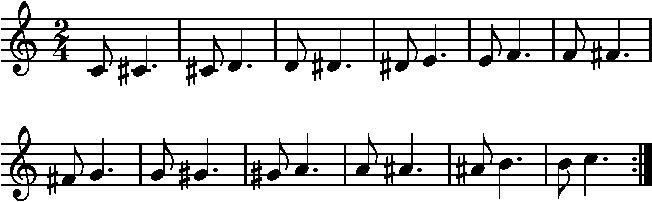
\includegraphics{scores/endless-cropped}
  \end{center}
  \pause
  De toonladder \alert{herhaalt} zich, zonder overgang!
\end{frame}

\begin{frame}
  \frametitle{Wat is er aan de hand?}

  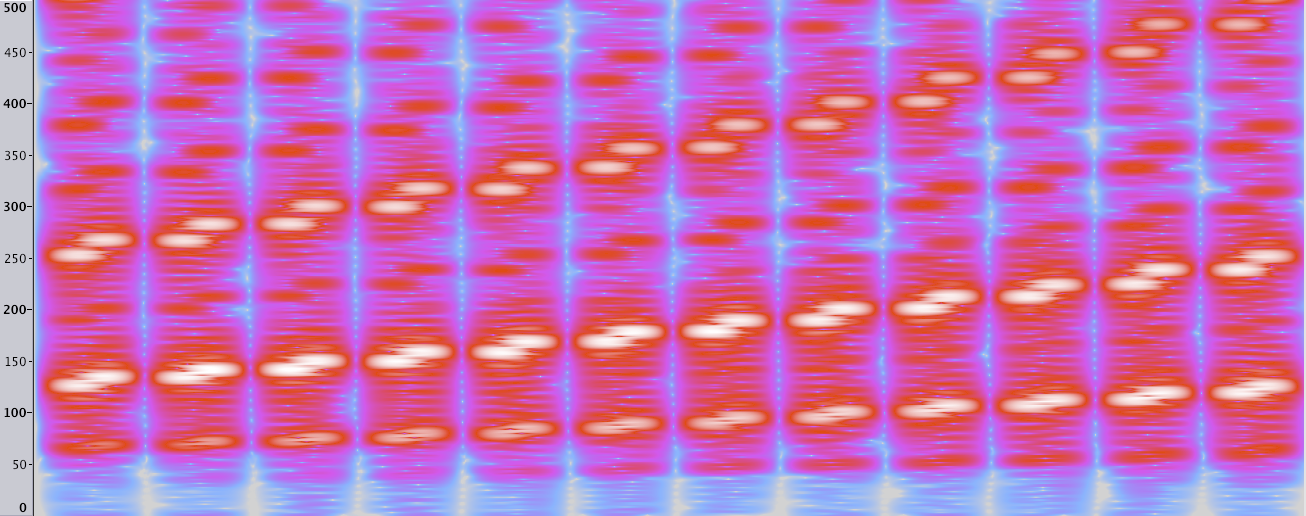
\includegraphics[width=\textwidth]{images/endless-once.png}
\end{frame}

\begin{frame}
  \frametitle{Observaties}

  \begin{enumerate}
    \item (alles is een beetje te laag gestemd)
    \item er is geen vastomlijnde grondtoon
    \item de duidelijkste frequentie wordt \alert{zwakker}
    \item de nauwelijks aanwezige laagste frequentie wordt \alert{sterker}
    \item de laatste toon heeft dezelfde samenstelling als de eerste
  \end{enumerate}
\end{frame}

\begin{frame}
  \frametitle{Paradox van Shepard}

  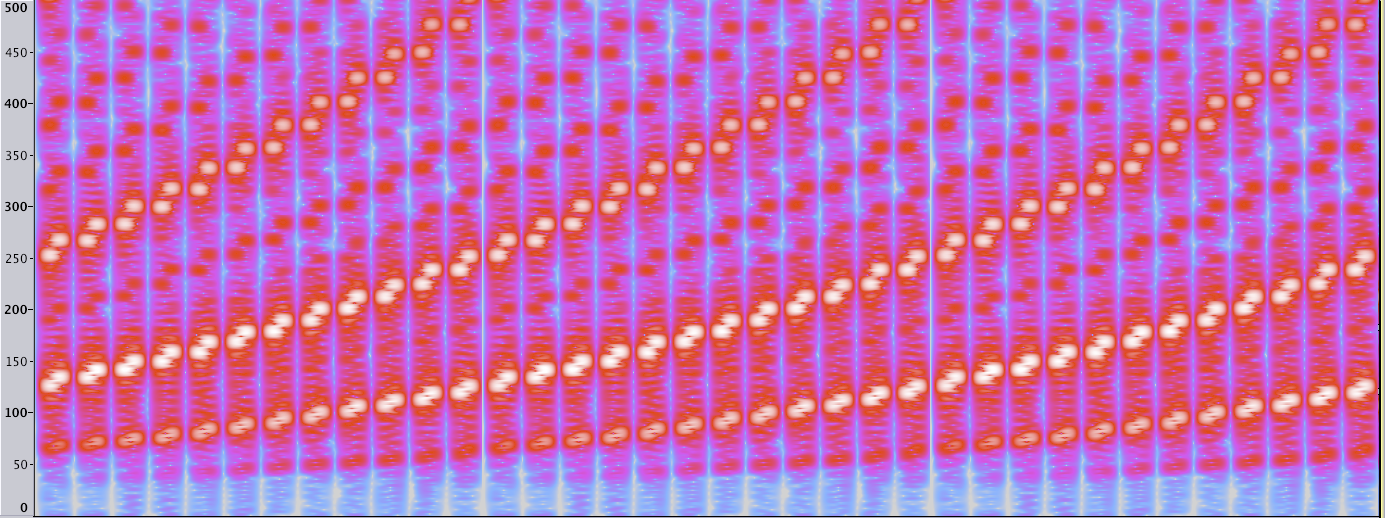
\includegraphics[width=\textwidth]{images/endless-copies.png}

  \begin{block}{Toepassing}
    Bassen op een klein membraan.
  \end{block}
\end{frame}

\begin{frame}
  \frametitle{Een oneindig dalende glissando}

  Een continue versie van voorgaande paradox
  \begin{block}{\twonotes\ audiofragment}
    \texttt{samples/shepard-risset-glissando.ogg}
  \end{block}
\end{frame}

\begin{frame}
  \frametitle{Paradox van Shepard--Risset}

  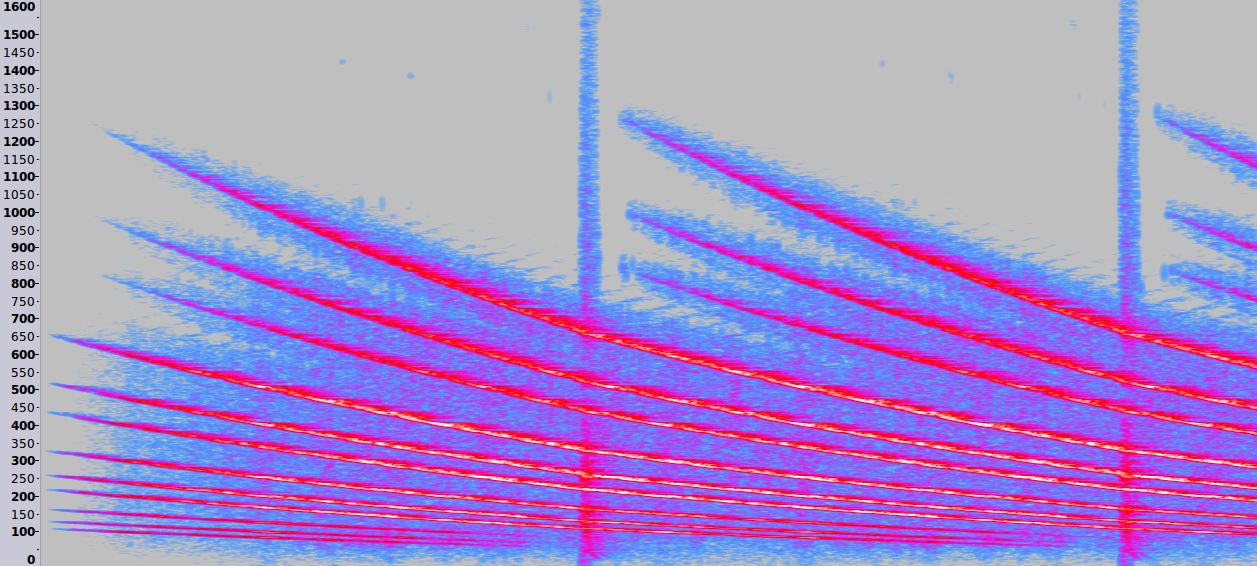
\includegraphics[width=\textwidth]{images/glissando-spectrum.png}
\end{frame}

\begin{frame}
  \frametitle{Een oneindig versnellende beat}

  \begin{block}{\twonotes\ audiofragment}
    \texttt{samples/drumbeat.ogg}
  \end{block}

  \begin{enumerate}
    \item we versnellen de hele tijd
    \item de snelste noten worden zachter
    \item de traagste worden sterker
  \end{enumerate}
  \pause
  \begin{block}{\twonotes\ audiofragment}
    \texttt{samples/drumbeat.ogg} met willekeurig doorspoelen
  \end{block}
\end{frame}

\end{document}

